\documentclass[10pt]{article}

\usepackage[margin=0.75in]{geometry}
\usepackage{amsmath,amsthm,amssymb}
\usepackage{xcolor}
\usepackage{cancel}
\usepackage{graphicx}
\usepackage{changepage}
\usepackage{circuitikz}
\usepackage{pgfplots}
\usepackage{subcaption}
\usepackage{physics}
\usepackage{siunitx}
\usepackage{minted}
\usepackage[breakable]{tcolorbox}
\usepackage[inline]{enumitem}

\theoremstyle{definition}
\newtheorem{problem}{Problem}
\newtheorem{soln}{Solution}

\pgfplotsset{compat=newest}
\usetikzlibrary{lindenmayersystems}
\usetikzlibrary{arrows}

\definecolor{incolor}{HTML}{303F9F}
\definecolor{outcolor}{HTML}{D84315}
\definecolor{cellborder}{HTML}{CFCFCF}
\definecolor{cellbackground}{HTML}{F7F7F7}
\newcommand{\eq}{=}
\tikzset
{%
  axes/.style={thick,-latex},
  cylinder/.style={right color=blue!80,left color=white,fill opacity=0.7},
  paraboloid back/.style={left color=magenta!80,fill opacity=0.4},
  paraboloid front/.style={left color=white, right color=magenta!80,fill opacity=0.4},
}

\usetikzlibrary{angles,
                backgrounds,
                decorations.pathmorphing,
                    calligraphy,% had to be after decorations.pathreplacing
                patterns.meta,
                quotes,
                patterns,
                snakes}

                \colorlet{xcol}{blue!70!black}
                \colorlet{darkblue}{blue!40!black}
                \colorlet{myred}{red!65!black}
                \tikzstyle{mydashed}=[xcol,dashed,line width=0.25,dash pattern=on 2.2pt off 2.2pt]
                \tikzstyle{axis}=[->,thick] %line width=0.6
                \tikzstyle{ell}=[{Latex[length=3.3,width=2.2]}-{Latex[length=3.3,width=2.2]},line width=0.3]
                \tikzstyle{dx}=[-{Latex[length=3.3,width=2.2]},darkblue,line width=0.3]
                \tikzstyle{ground}=[preaction={fill,top color=black!10,bottom color=black!5,shading angle=20},
                                    fill,pattern=north east lines,draw=none,minimum width=0.3,minimum height=0.6]
                \tikzstyle{mass}=[line width=0.6,red!30!black,fill=red!40!black!10,rounded corners=1,
                                  top color=red!40!black!20,bottom color=red!40!black!10,shading angle=20]
                \tikzstyle{spring}=[line width=0.8,blue!7!black!80,snake=coil,segment amplitude=5,segment length=5,line cap=round]
                \tikzset{>=latex} % for LaTeX arrow head
                \tikzstyle{force}=[->,myred,very thick,line cap=round]
                \def\tick#1#2{\draw[thick] (#1)++(#2:0.1) --++ (#2-180:0.2)}                

\makeatletter
\newcommand{\boxspacing}{\kern\kvtcb@left@rule\kern\kvtcb@boxsep}
\makeatother
\newcommand{\prompt}[4]{
    \ttfamily\llap{{\color{#2}[#3]:\hspace{3pt}#4}}\vspace{-\baselineskip}
}

\newcommand{\highlight}[1]{\colorbox{yellow}{$\displaystyle #1$}}

\newcommand{\volts}[0]{\mathrm{V}}
\newcommand{\amps}[0]{\mathrm{A}}
\newcommand{\ohms}[0]{\Omega}
\newcommand{\farad}[0]{\mathrm{F}}
\newcommand{\coulomb}[0]{\mathrm{C}}
\newcommand{\watts}[0]{\mathrm{W}}

\newcommand{\ihat}{\boldsymbol{\hat{\imath}}}
\newcommand{\jhat}{\boldsymbol{\hat{\jmath}}}

\NewDocumentCommand{\evalat}{sO{\big}mm}{%
  \IfBooleanTF{#1}
   {\mleft. #3 \mright|_{#4}}
   {#3#2|_{#4}}%
}

\title{Physics 2130: Assignment 1}
\author{Jeremy Favro}
\date{\today}

\begin{document}

\maketitle

% PROBLEM 1
\begin{problem}
A particle moving in two dimensions has an acceleration:
\begin{align*}
     {a} = \left[-\frac{3}{1+t}\ihat+20\cos(5t)\jhat\right]
\end{align*} \\
where $t$ is measured in seconds. The particle starts from rest at the origin.
\end{problem}
\begin{soln}
     Initial conditions are that $\int \int {a}(t=0) \,dt \,dt=0$ and $\int {a}(t=0) \,dt=0$.
     a) Finding $x(t)$ (position in the $\ihat$ direction)
     \begin{align*}
           & = \int \int -\frac{3}{1+t} \,dt\,dt                                                                                \\
           & = -3\int \int \frac{1}{1+t} \,dt\,dt \rightsquigarrow \mathrm{ let} \, u=1+t \implies\frac{du}{dt}=1\implies du=dt \\
           & = -3\int \int \frac{1}{u} \,du\,dt                                                                                 \\
           & = -3\int \ln(u) \,dt                                                                                               \\
           & = -3\int \ln(1+t) \,dt \rightsquigarrow \mathrm{ let} \, u=1+t \implies\frac{du}{dt}=1\implies du=dt               \\
           & = -3\int \ln(u) \,du                                                                                               \\
           & = -3u\left[\ln(u)-1\right] + C                                                                                     \\
           & = -3(1+t)\left[\ln(1+t)-1\right] + C
     \end{align*}
     At $x(t=0)=0$ thus
     \begin{align*}
           & -3(1+0)\left[\cancelto{0}{\ln(1+0)}-1\right] + C=0 \\
           & 3 + C=0                                            \\
           & C=-3
     \end{align*}
     $\therefore x(t)= -3(1+t)\left[\ln(1+t)-1\right] - 3$ \\
     Next finding Finding $y(t)$ (position in the $\jhat$ direction)
     \begin{align*}
           & = \int \int 20\cos(5t) \,dt\,dt                                                                                         \\
           & = 20\int \int \cos(5t) \,dt\,dt \rightsquigarrow \mathrm{ let} \, u=5t \implies\frac{du}{dt}=5\implies \frac{1}{5}du=dt \\
           & = 4\int \int \cos(u) \,du\,dt                                                                                           \\
           & = 4\int \sin(5t)\,dt \rightsquigarrow \mathrm{ let} \, u=5t \implies\frac{du}{dt}=5\implies \frac{1}{5}du=dt            \\
           & = 4\int \sin(u)\,dt \rightsquigarrow \mathrm{ let} \, u=5t \implies\frac{du}{dt}=5\implies \frac{1}{5}du=dt             \\
           & = -\frac{4}{5}\cos(5t) + C                                                                                              \\
     \end{align*}
     At $y(t=0)=0$ thus
     \begin{align*}
           & -\frac{4}{5}\cos(\cancelto{0}{5t}) + C = 0 \\
           & -\frac{4}{5} + C = 0                       \\
           & C=\frac{4}{5}
     \end{align*}
     $\therefore y(t) = -\frac{4}{5}\cos(5t) + \frac{4}{5}$ \\
     b) \\
     \begin{figure}[h]
          \begin{subfigure}[t]{0.49\textwidth}
               \vspace{-27pt}
               \includegraphics[width=\textwidth]{Figure_1.png}
          \end{subfigure}\hfill
          \begin{subfigure}[t]{0.49\textwidth}
               \begin{minted}[fontsize=\footnotesize, breaklines, autogobble]{python}
               import matplotlib.pyplot as pyplot
               import numpy as np
     
               t=np.arange(0,3,0.01)
               def x(t):
                    return -3*(1+t)*(np.log(1+t)-1) - 3
               def y(t):
                    return -(4/5)*np.cos(5*t) + 4/5 # Note: numpy trig takes radians!!!
     
               pyplot.plot(x(t),y(t))
               pyplot.show()
         \end{minted}
          \end{subfigure}%
     \end{figure}
\end{soln}

% PROBLEM 2
\begin{problem}
Assume that a projectile of mass $m$ is short with initial speed $v_0$ and angle $\theta$ from an initial height $h_0$
\end{problem}
\begin{soln} ~\\
     a)
     \begin{align*}
           & F_x=\cancel{m}\ddot{x}=-k\cancel{m}v                                                                    \\
           & \Rightarrow \frac{dv_x}{dt}=-kv_x                                                                       \\
           & \Rightarrow \int \frac{1}{v_x} \,dv_x = -k\int\,dt                                                      \\
           & \Rightarrow \ln \abs{v_x} = -kt+C \rightsquigarrow v_x(t=0)=v_0\cos\theta \implies \ln(v_0\cos\theta)=C \\
           & \Rightarrow v_x = e^{-kt}e^{\ln(v_0\cos\theta)}                                                         \\
           & \therefore v_x(t) = (v_0\cos\theta)e^{-kt}                                                              \\
     \end{align*}

     \begin{align*}
           & F_y=\cancel{m}\ddot{y}=-\cancel{m}g-k\cancel{m}v                                                                                   \\
           & \Rightarrow \frac{dv_y}{dt}=-g-kv_y                                                                                                \\
           & \Rightarrow \int \frac{1}{g+kv_y} \,dv_y = -\int\,dt                                                                               \\
           & \Rightarrow \frac{1}{k}\ln \abs{g+kv_y} = -t+C \rightsquigarrow v_y(t=0)=v_0\sin\theta \implies \frac{1}{k}\ln(g+kv_0\sin\theta)=C \\
           & \Rightarrow g + kv_y = e^{-kt}e^{\ln(g+kv_0\sin\theta)}                                                                            \\
           & \therefore v_y(t) = \frac{1}{k}(g+kv_0\sin\theta)e^{-kt}-\frac{g}{k}                                                               \\
     \end{align*}
     b) \begin{align*}
           & x(t)=\int v_x(t) \,dt                                                                                 \\
           & = \int (v_0\cos\theta)e^{-kt} \,dt                                                                    \\
           & = -\frac{1}{k}(v_0\cos\theta)e^{-kt}+C\rightsquigarrow x(t=0)=0 \implies C=\frac{1}{k}(v_0\cos\theta) \\
           & \therefore x(t)=\frac{(v_0\cos\theta)}{k}\left[1-e^{-kt}\right]
     \end{align*}

     \begin{align*}
           & y(t)=\int v_y(t) \,dt                                                                                                                                                          \\
           & =\int \frac{1}{k}(g+kv_0\sin\theta)e^{-kt}-\frac{g}{k} \,dt                                                                                                                    \\
           & = -\frac{1}{k^2}(g+kv_0\sin\theta)e^{-kt}-\frac{gt}{k} + C \rightsquigarrow y(t=0)=h_0 \implies C=h_0+\frac{1}{k^2}(g+kv_0\sin\theta)                                          \\
           & \therefore y(t) = -\frac{1}{k^2}(g+kv_0\sin\theta)e^{-kt}-\frac{gt}{k} + h_0 + \frac{1}{k^2}(g+kv_0\sin\theta) = \frac{1}{k^2}(g+kv_0\sin\theta)(1-e^{-kt}) + h_0-\frac{gt}{k} \\
     \end{align*}

     c) \begin{align*}
           & y(t=t_f)=0=\frac{1}{k}(g+kv_0\sin\theta)(1-e^{-kt_f}) + h_0 \\
           & -h_f=\frac{1}{k}(g+kv_0\sin\theta)(1-e^{-kt_f})             \\
           & -\frac{h_fk}{g+kv_0\sin\theta}-1=e^{-kt_f}                  \\
           & -\frac{1}{k}\ln(-\frac{h_fk}{g+kv_0\sin\theta}-1)=t_f       \\
     \end{align*}
     \begin{align*}
           & R=x(t=t_f)=\frac{(v_0\cos\theta)}{k}\left[1-e^{\ln(-\frac{h_fk}{g+kv_0\sin\theta}-1)}\right] \\
     \end{align*}
     d) \\
     \begin{figure}[h]
          \begin{subfigure}[t]{0.49\textwidth}
               \vspace{-27pt}
               \includegraphics[width=\textwidth]{Figure_2.png}
          \end{subfigure}\hfill
          \begin{subfigure}[t]{0.49\textwidth}
               \begin{minted}[fontsize=\footnotesize, breaklines, autogobble]{python}
                    import matplotlib.pyplot as pyplot
                    import numpy as np

                    m = 1
                    v_0 = 600
                    h_0 = 500
                    theta = 60 * (np.pi/180)
                    g = 9.81
                    k_vals = [0, 0.02, 0.04, 0.06]

                    t = np.arange(0, 10, 0.01)

                    def x(t, k):
                         return (v_0*np.cos(theta))*t if k == 0 else ((v_0*np.cos(theta))/k)*(1-np.e**(-k*t)) # k=0 is a special case where there is no drag so we use the plain kinematic equation

                    def y(t, k):
                         return h_0 + (v_0*np.sin(theta))*t - (1/2)*g*t**2 if k == 0 else (1/k**2)*(g+k*v_0*np.sin(theta))*(1-np.e**(-k*t)) + h_0 - (g*t**2)/k

                    for k in k_vals:
                         pyplot.plot(x(t, k), y(t, k), label=f"k={k}")
    
                    pyplot.legend()
                    pyplot.ylim(bottom=0, top=2000)
                    pyplot.xlabel("x (m)")
                    pyplot.ylabel("y (m)")
                    pyplot.show()
               \end{minted}
          \end{subfigure}%
     \end{figure}
\end{soln}

% PROBLEM 3
\begin{problem}
To practice his skills, an archer is shooting at a rubber duck located on top of a wooden fence. The fence is
located at a distance $x_d=45\unit{\meter}$ away, and it stands $h_d=1.5\unit{\meter}$ tall. The archer is shooting at an angle of $\theta=35\unit{\degree}$ holding
the bow at a height of $h_0=1.2\unit{\meter}$ from the ground. \\
Determine the initial velocity needed for the arrow to hit the duck. Ignore air resistance. (Note: start from Newton's equations and show your work)
\end{problem}
\begin{soln} Note: I defined some variables in the problem statement \\
     \begin{center}
          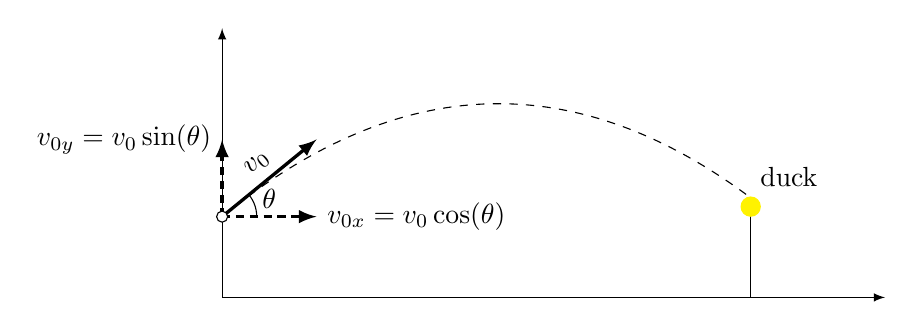
\begin{tikzpicture}[scale=1, transform shape]  %projectile motion
               \begin{axis}[
                         width=10cm, %set bigger width
                         height=5cm,
                         xmin=0,xmax=11.5,
                         ymin=0,ymax=4,
                         % xlabel style={anchor=east},
                         % ylabel style={anchor=north},
                         % anchor=north,
                         % xlabel=$x$,
                         % ylabel=$y$,
                         axis x line = bottom,
                         axis y line = left,
                         axis line style={->},
                         %axis on top,
                         ticks = none,clip=false,
                    ]

                    \tikzset{every mark/.append style={fill=white}}

                    %variable definitions
                    \def\g{-9.8} %gravity
                    \def\v{10} %velocity
                    \def\ang{35} %angle
                    \def\s{0.2}
                    \pgfmathsetmacro{\t}{0}
                    %flight path
                    \addplot[
                         dashed,
                         domain=0:9.17,
                         samples=100,]
                    {{\g*(x^2)/(2*\v^2*cos(\ang)^2)+x*tan(\ang)+1.2}};

                    %vector at start
                    \coordinate (A) at (axis cs: {\v*cos(\ang)*\t}, {\v*\t*sin(\ang)+0.5*\g*(\t^2)+1.2});
                    \coordinate (B) at (axis cs: {\v*cos(\ang)*\t+\s*\v*cos(\ang)}, {\v*\t*sin(\ang)+0.5*\g*\t^2+\s*(\v*sin(\ang)+\g*\t)+1.2});
                    \draw[very thick,->](A)--(B)
                    node[midway,sloped,above]{${v_0}$};
                    \draw[densely dashed,very thick,->](A)--(B|-A)
                    node[below,right]{$v_{0x}={v_0}\cos(\theta)$};
                         \draw[densely dashed,very thick,->](A)--(B-|A)
                         node[above,left]{$v_{0y}={v_0}\sin(\theta)$};

                    \path plot[mark=*] coordinates {(A)};

                    %dashed box around start vector
                    % \draw[dashed](B-|A)--(B);
                    % \draw[dashed](B|-A)--(B);

                    %fence
                    \draw [arrows = {-Circle[yellow,scale=2]}](9.17,0) -- (9.17,1.5) node[above right] {duck};

                    %start vector angle label
                    \node[circle,minimum size=25pt] at (A) (circ) {};
                    \node[right] at (circ.30) {$\theta$};
                    \path[clip] (A) -- (B) -- (B|-A) -- cycle;
                    \node[circle,draw,minimum size=25pt] at (A) (circ) {};
               \end{axis}
          \end{tikzpicture}
     \end{center}
     Using Newton's equations
     \begin{align*}
           & F_x=m\ddot{x}=0                                                                               \\
           & \Rightarrow\displaystyle\frac{dv_x}{dt}=0                                                     \\
           & \Rightarrow dv_x=0                                                                            \\
           & \Rightarrow\int 1 \,dv_x = \int 0 \,dt                                                        \\
           & \Rightarrow v_x(t)=0+C \rightsquigarrow v_x(t=0)=0+{v_0}\cos\theta \implies C={v_0}\cos\theta \\
           & \therefore v_x(t)={v_0}\cos\theta                                                             \\
     \end{align*}
     \begin{align*}
           & x(t)=\int v_x(t) \,dt                                                                               \\
           & =\int {v_0}\cos\theta \,dt                                                                          \\
           & =({v_0}\cos\theta)t + C \rightsquigarrow x(t=0)=0=\cancelto{0}{({v_0}\cos\theta)t} + C \implies C=0 \\
           & \therefore x(t)=({v_0}\cos\theta)t                                                                  \\
     \end{align*}
     \par\noindent\rule{\textwidth}{0.4pt}
     \begin{align*}
           & F_y=\cancel{m}\ddot{y}=-\cancel{m}g                                                                    \\
           & \Rightarrow\displaystyle\frac{dv_y}{dt}=-g                                                             \\
           & \Rightarrow dv_y=-gdt                                                                                  \\
           & \Rightarrow\int 1 \,dv_y = \int -g \,dt                                                                \\
           & \Rightarrow v_y(t)=-gt+C \rightsquigarrow v_y(t=0)=-g\cdot0+{v_0}\sin\theta \implies C={v_0}\sin\theta \\
           & \therefore v_y(t)=-gt+{v_0}\sin\theta                                                                  \\
     \end{align*}
     \begin{align*}
           & y(t)=\int v_y(t) \,dt                                                                                                                             \\
           & =\int -gt+{v_0}\sin\theta \,dt                                                                                                                    \\
           & =-\frac{gt^2}{2}+({v_0}\sin\theta)t+C \rightsquigarrow y(t=0)=h_0=\cancelto{0}{-\frac{gt^2}{2}}+\cancelto{0}{({v_0}\sin\theta)t}+C \implies C=h_0 \\
           & \therefore y(t)=-\frac{gt^2}{2}+({v_0}\sin\theta)t+h_0                                                                                            \\
     \end{align*}
     Now we have two equations $x(t)$ and $y(t)$ with two unknowns which can be solved to determine ${v_0}$. Solving $x(t)$ for $t$ yields $t_{f}=\displaystyle\frac{x_d}{{v_0}\cos\theta}$.
     Substituting into $y(t)$
     \begin{align*}
           & y(t=t_{f})=h_d=-\frac{g\left(\frac{x_d}{{v_0}\cos\theta}\right)^2}{2}+({v_0}\sin\theta)\left(\frac{x_d}{{v_0}\cos\theta}\right)+h_0      \\
           & h_d-h_0=-\frac{g\left(\frac{x_d}{{v_0}\cos\theta}\right)^2}{2}+\left(\frac{x_d\cancel{{v_0}}\sin\theta}{\cancel{{v_0}}\cos\theta}\right) \\
           & h_d-h_0=-\frac{g\left(\frac{x_d}{{v_0}\cos\theta}\right)^2}{2}+x_d\tan\theta                                                             \\
           & 2\left(h_d-h_0-x_d\tan\theta\right)=-g\left(\frac{x_d}{{v_0}\cos\theta}\right)^2                                                         \\
           & -\frac{2}{g}\left(h_d-h_0-x_d\tan\theta\right)=\frac{x_d^2}{{v_0}^2\cos^2\theta}                                                         \\
           & -\frac{2\cos^2\theta}{gx_d^2}\left(h_d-h_0-x_d\tan\theta\right)=\frac{1}{{v_0}^2}                                                        \\
           & \sqrt{\left[-\frac{2\cos^2\theta}{gx_d^2}\left(h_d-h_0-x_d\tan\theta\right)\right]^{-1}}={v_0}                                           \\
           & v_0=19.7\unit{\meter\per\second}\text{ 35\unit{\degree} above the horizontal }                                                           \\
     \end{align*}
\end{soln}

% PROBLEM 4
\begin{problem}
A block of mass $m$ is at rest on top of a slope that forms an angle $\theta$ with the horizontal. At time $t=0\unit{\second}$, the block
is let go down the slope. Note that the slope has a coefficient of friction $\mu_f$ and the block also experiences a drag proportional to the speed $\abs{F_d}=\tilde{k}v$.
\end{problem}
\begin{soln} ~\\
     \begin{center}
          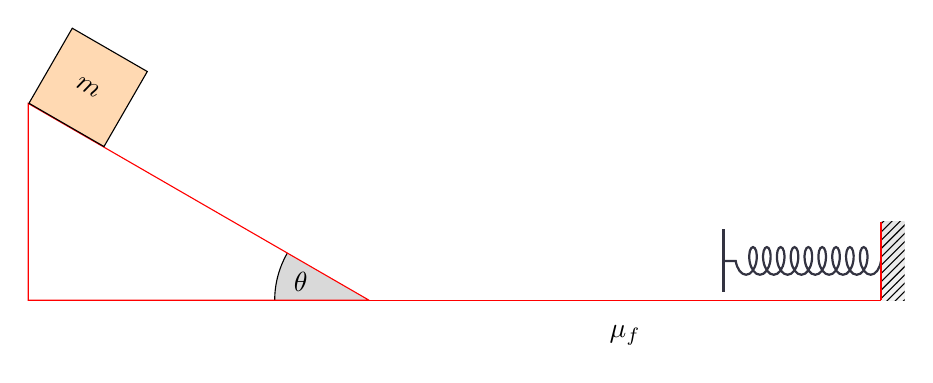
\begin{tikzpicture}[
                    ANG/.style = {draw, fill=gray!30,
                              angle radius = 12mm,
                              angle eccentricity=0.75},
                    BC/.style args = {#1/#2/#3}{
                              decorate,
                              decoration={calligraphic brace, amplitude=6pt,
                                        pre =moveto, pre  length=1pt,
                                        post=moveto, post length=1pt,
                                        raise=#1,
                                        #2},% for mirroring of brace
                              very thick,
                              pen colour={#3}},
                    N/.style = {draw, fill=orange!30, minimum size=11mm,
                              anchor=south west}
               ]
               \def\Ang{150}
               \draw[red]  (3.5,0)  coordinate[] (b) -- ++   % <---
               (\Ang:5) coordinate[] (a) |-
               (b)      coordinate[pos=0.5] (c);
               \scoped[on background layer]
               \pic [ANG, "$\theta$"]  {angle = a--b--c};
               %
               \node[N, rotate around={330:(a)}] at (a) {$m$};
               % new
               \draw[red]  (b) -- node[below=2mm, black] {$\mu_f$} ++ (6.5,0) coordinate[] (aux);


               \def\H{1}    % wall height
               \def\T{0.3}  % wall thickness
               \def\W{2.6}  % ground length
               \def\D{0.25} % ground depth
               \def\h{0.6}  % mass height
               \def\w{0.7}  % mass width
               \def\x{1.6}  % mass x position
               \draw[spring] (10,0.5) -- (8,.5);
               \draw[ground] (10.3,0) |-++ (-\T,\H) -- (10,0) -- cycle;
               \draw[red] (10,\H) -- (10,0) ;
               \draw[blue!7!black!80, thick] (8,\H-0.1) -- (8,0.1) ;

               % \draw (0,\H) -- (0,0) -- (\W,0);
               % \draw[mass] (\x,0) rectangle++ (\w,\h) node[midway] {$m$};

          \end{tikzpicture}
     \end{center}
     a)
     \begin{align*}
           & F_x=\cancel{m}\ddot{x}=\cancel{m}g\sin\theta-\mu \cancel{m}g\cos\theta - k\cancel{m}v_x                                                                      \\
           & \Rightarrow \frac{dv_x}{dt}=g\sin\theta-\mu g\cos\theta - kv_x                                                                                               \\
           & \Rightarrow \int \frac{1}{g\sin\theta-\mu g\cos\theta - kv_x}\,dv_x= \int  \,dt                                                                              \\
           & \Rightarrow -\frac{1}{k}\ln(g\sin\theta-\mu g\cos\theta - kv_x) = t + C \rightsquigarrow v_x(t=0)=0 \implies C=-\frac{1}{k}\ln(g\sin\theta-\mu g \cos\theta) \\
           & \Rightarrow -\frac{1}{k}\ln(g\sin\theta-\mu g\cos\theta - kv_x) = t - \frac{1}{k}\ln(g\sin\theta-\mu g \cos\theta)                                           \\
           & \Rightarrow \ln(g\sin\theta-\mu g\cos\theta - kv_x) = -kt + \ln(g\sin\theta-\mu g \cos\theta)                                                                \\
           & \Rightarrow g\sin\theta-\mu g\cos\theta - kv_x = (g\sin\theta-\mu g \cos\theta)e^{-kt}                                                                       \\
           & \Rightarrow - kv_x = (g\sin\theta-\mu g \cos\theta)e^{-kt} + \mu g\cos\theta -g\sin\theta                                                                    \\
           & \therefore v_x = -\frac{1}{k}((g\sin\theta-\mu g \cos\theta)e^{-kt} + \mu g\cos\theta -g\sin\theta)                                                          \\
     \end{align*}

     \begin{align*}
           & F_y=\cancel{m}\ddot{y}=0                                     \\
           & \Rightarrow\frac{dv_y}{dt}=0                                 \\
           & \Rightarrow v_y=0+C \rightsquigarrow v_y(t=0)=0 \implies C=0 \\
           & \therefore v_y(t)=0                                          \\
     \end{align*}
     b) After a long time the block reaches its terminal velocity of approx. $10\unit{\meter\per\second}$. The block never reaches $40\unit{\meter\per\second}$ because that is more than the terminal velocity
     ~\\\begin{figure}[h]
          \begin{subfigure}[t]{0.49\textwidth}
               \vspace{-27pt}
               \includegraphics[width=\textwidth]{Figure_3.png}
          \end{subfigure}\hfill
          \begin{subfigure}[t]{0.49\textwidth}
               \begin{minted}[fontsize=\footnotesize, breaklines, autogobble]{python}
                    import matplotlib.pyplot as pyplot
                    import numpy as np

                    max_time = 80
                    theta = 45 * (np.pi/180)
                    g = 9.81
                    mu = 0.5
                    k = 0.6
                    m = 10

                    t = np.arange(0,max_time,0.01)

                    N = g*np.cos(theta)

                    def v_x(t):
                         return (-1/k)*((g*np.sin(theta)-mu*N)*np.e**(-k*t)
                         +mu*N-g*np.sin(theta))

                    pyplot.plot(t, v_x(t))
                    pyplot.xlabel("Time (s)")
                    pyplot.ylabel("Velocity (m/s)")
                    pyplot.show()
               \end{minted}
          \end{subfigure}%
     \end{figure} ~\\
     c)
     \begin{align*}
           & F_x=\cancel{m}\ddot{x}=-\mu \cancel{m}g                                                        \\
           & \Rightarrow \frac{dv_x}{dx}\frac{dx}{dt}=-\mu g                                                \\
           & \Rightarrow v_x\frac{dv_x}{dx}=-\mu g                                                          \\
           & \Rightarrow \frac{v_x^2}{2}=-\mu gx+C \rightsquigarrow v_x(x=0)=v_e \implies C=\frac{v_e^2}{2} \\
           & \Rightarrow \frac{v_x^2}{2}=-\mu gx+\frac{v_e^2}{2}                                            \\
           & \Rightarrow v_x^2=-2\mu gx+v_e^2                                                               \\
           & \therefore v_x=\sqrt{v_e^2-2\mu gx}                                                            \\
     \end{align*}
     Now, by conservation of energy
     \begin{align*}
           & E_{tot}=E_{tot}^\prime                           \\
           & \frac{1}{2}m(v_e^2-2\mu gd)=\frac{1}{2}\beta x^2 \\
           & m(v_e^2-2\mu gd)=\beta x^2                       \\
           & \sqrt{\frac{m}{\beta}(v_e^2-2\mu gd)}=x          \\
     \end{align*}
     Note: this checks out by the first tenet of ``street fighting physics'', dimensional analysis, which is good because I don't feel confident in it. I've been looking at all of these equations
     for too long.
\end{soln}

% PROBLEM 5
\begin{problem}
An object is tossed vertically down a cliff with initial speed $v_0$. Besides gravity, it experiences a resisting, drag
force that is proportional to the square of the velocity (i.e., $kmv^2$). Show that the distance travelled as the object
accelerates from the initial speed $v_0$ to the final speed $v_1$ is given by the expression:
$$\frac{1}{2k}\ln\abs{\frac{g-kv_0^2}{g-kv_1^2}}$$
\end{problem}
\begin{soln} We're looking for an expression of position in terms of velocity which we can get using the so-called ``fuckery with the differentials'' which still confuses me.
     \begin{align*}
           & \ddot{x} = -g+kv^2 \rightsquigarrow \text{ I'm using the ``wrong'' axis here because it's what I chose initially}                                                                                           \\
           & \frac{dv}{dt} = -g+kv^2                                                                                                                                                                                     \\
           & \highlight{\frac{dv}{dx}}\frac{dx}{dt} = -g+kv^2 \rightsquigarrow \text{ Here's where the } x\propto v \text{ comes up}                                                                                     \\
           & v\frac{dv}{dx} = -g+kv^2                                                                                                                                                                                    \\
           & \frac{v}{-g+kv^2}dv = dx                                                                                                                                                                                    \\
           & \int \frac{v}{-g+kv^2} \,dv = x + C \rightsquigarrow C \text{ will be zero here as } v_0, x_0 = 0                                                                                                           \\
           & \frac{1}{2k}\int \frac{\cancel{v}}{s\cancel{v}} \,ds = x \rightsquigarrow s=-g+kv^2 \text{ because I can't tell the difference between $u$ and $v$ in my handwriting}                                       \\
           & x(v)=\frac{1}{2k}\ln\left(kv^2-g\right) \implies \eval{x(v)}_{v_1}^{v_0}=\Delta x=\frac{1}{2k}\left[\ln\left(kv_0^2-g\right)-\ln\left(kv_1^2-g\right)\right]=\frac{1}{2k}\ln\abs{\frac{kv_0^2-g}{kv_1^2-g}} \\
     \end{align*}
     Which, as noted at the beginning is ``wrong'' because I used the opposite axis (negative down).
\end{soln}
\end{document}